\chapter{Multithreading in Java}
I thread sono \textbf{astrazioni del linguaggio}.
\\Diversi modelli in base all'astrazione che vogliamo.

\section{Java threads}
Sono astrazioni offerte della JVM e gestiti dalla stessa.
\\Tipicamente implementati sfruttando il modello di threading offerto dal sistema operativo (ma lo standard JVM non specifica come).
\\La JVM offre quindi una libreria per la definizione dei thread e per l'interazione con il Sistema Operativo per la loro esecuzione.
\\Modalità principali di creazione dei thread in Java:
\begin{itemize}
    \item Sottoclasse della classe standard \verb#java.lang.Thread#
    \item (Meglio) Implementazione metodo \verb#run()# interfaccia \verb#java.lang.Runnable#
\end{itemize}

\subsection{Il thread main}
In Java ogni programma in esecuzione è un thread,
\begin{itemize}
    \item Il metodo \verb#main()# è associato al thread «main»
    \item Per poter accedere alle proprietà del thread in esecuzione è necessario ottenerne un riferimento tramite il metodo \verb#currentThread()#
\end{itemize}
\begin{center}
    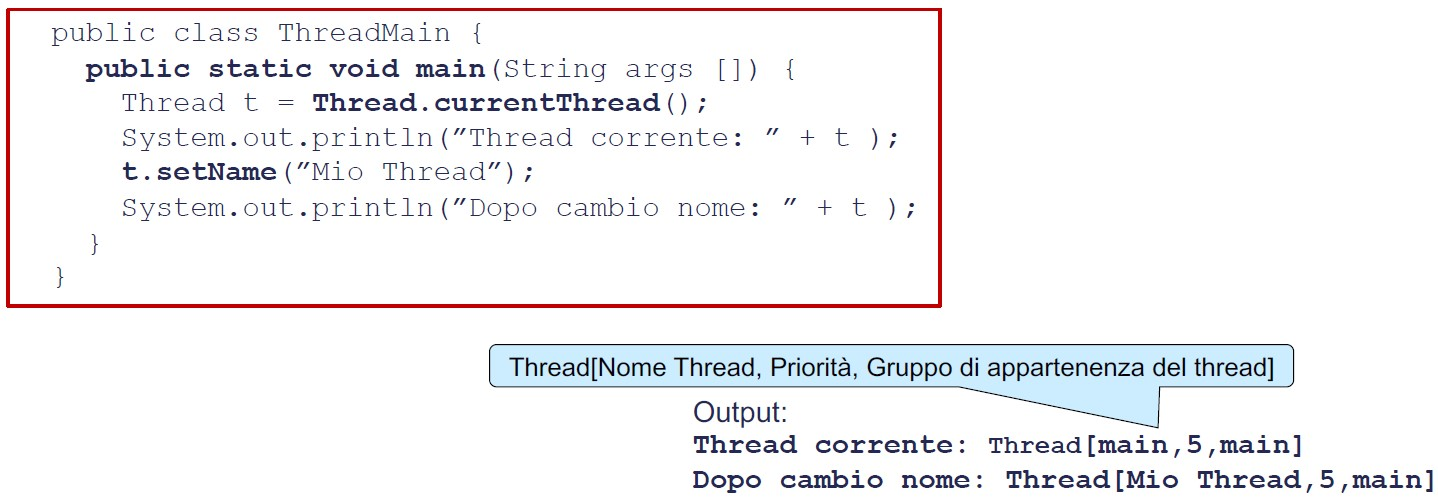
\includegraphics[width=0.75\textwidth]{img/thread_main1.jpg}
\end{center}

\subsection{La classe principale per i Thread in Java}
\begin{center}
    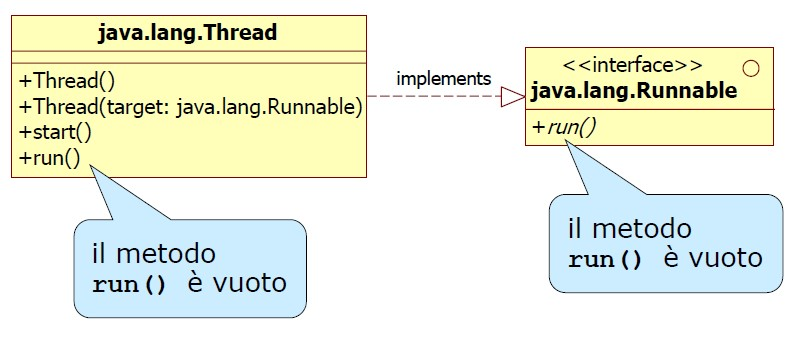
\includegraphics[width=0.675\textwidth]{img/thread1.jpg}
\end{center}
Il modo più semplice per creare ed eseguire un Thread è:
\begin{enumerate}
    \item Estendere la classe \verb#java.lang.Thread# (che contiene un metodo \verb#run()# vuoto)
    \item Riscrivere (ridefinire, \verb#override#) il metodo \verb#run()# nella sottoclasse.
    \\- Il codice eseguito dal thread è incluso nel metodo \verb#run()# e nei metodi invocati direttamente o indirettamente da \verb#run()#
    \\- Questo è il codice che verrà eseguito in parallelo a quello degli altri thread
    \item Creare un'istanza della sottoclasse
    \item Richiamare il metodo \verb#start()# su questa istanza
    \\NB: spesso si estende il costruttore in modo che questo invochi \verb#start()#: così creare l'istanza della sottoclasse fa anche partire il thread.
    \\Questo viene chiamato \textbf{Pattern} del Thread.
\end{enumerate}

\subsubsection{Estensione della classe Thread}
\begin{center}
    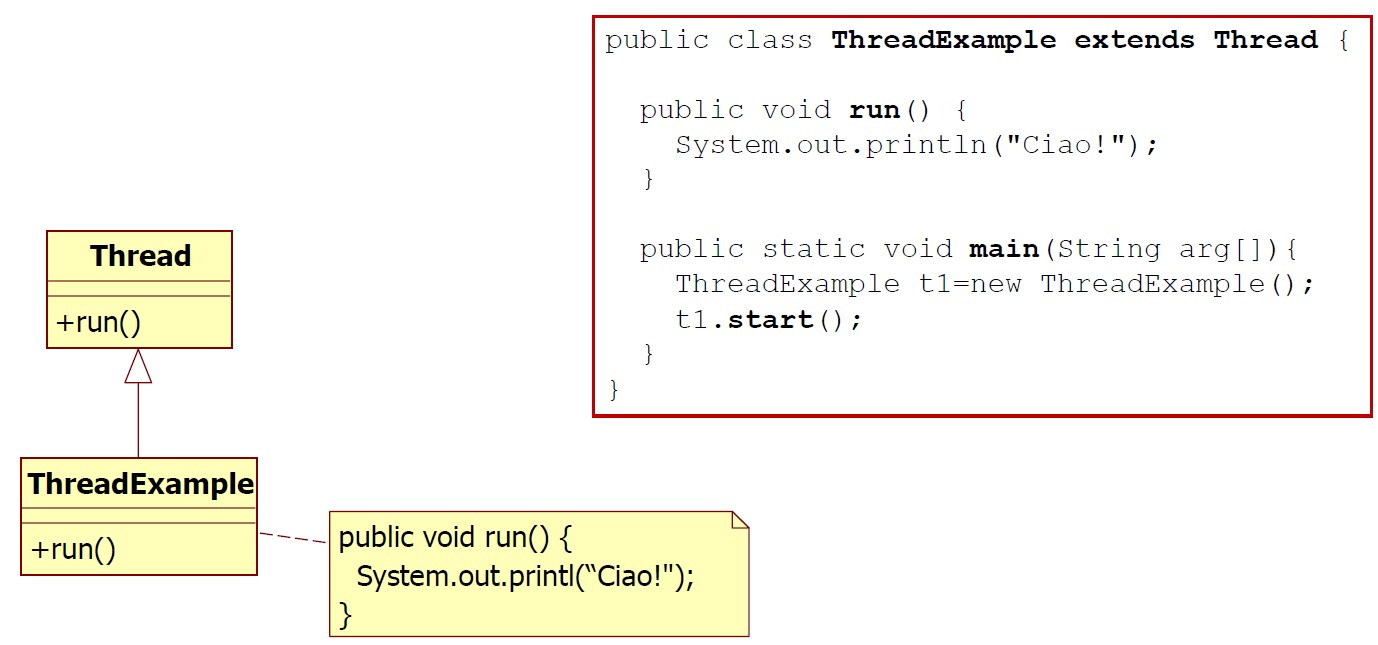
\includegraphics[width=0.675\textwidth]{img/thread2.jpg}
\end{center}
Domanda: quale thread termina per primo (sapendo che il main chiama un altro thread)?
\\Risposta: non possiamo saperlo, perché i thread non si attendono fra loro.

\subsection{Far partire i thread: start()}
\begin{itemize}
    \item Una chiamata \verb#t.start()# rende il thread \verb#t# pronto (ready) all'esecuzione.
    \\Chi chiama il metodo start? Il programmatore.
    \item Prima o poi (quando lo scheduler lo riterrà opportuno) il thread verrà mandato in esecuzione e verrà invocato il metodo \verb#run()# del thread t
    \\È importante notare che non dobbiamo chiamare esplicitamente il metodo run, la sua invocazione avviene in maniera automatica (è implementata internamente alla classe Thread)
    \item I due thread (creante e creato) saranno eseguiti in modo concorrente ed indipendente
    \\Una applicazione Java ha almeno un thread
    \item Importante:
    \\L'ordine con cui ogni thread eseguirà le proprie istruzioni è noto, ma l'ordine globale in cui le istruzioni dei vari thread saranno eseguite effettivamente è indeterminato (nondeterminismo)
\end{itemize}
Una delle conseguenze me la sono persa

\section{Runnable interface}
Siccome Java non consente l'ereditarietà multipla, un modo alternativo di realizzare un thread è implementare solamente il metodo run (ovvero implementare l'interfaccia Runnable), avendo la possibilità di estendere un'altra classe base (maggior flessibilità).
\\La classe base Thread (il cui metodo run non fa nulla) può essere inizializzata con un oggetto Runnable, del quale utilizzerà il metodo run una volta che viene fatta partire.
% img

\section{Thread: Alive o Terminated?}
Così abbiamo terminato la \textbf{creazione} di un thread. Ora lo dobbiamo usare.
L'invocazione del metodo start() porta il Thread ad eseguire il metodo \verb#run()# (l'entry point del thread):
\\- Un thread è considerato alive finché il metodo \verb#run()#non termina
\\- Quando \verb#run()#ritorna, il thread è considerato terminated
\\Una volta che un thread è terminato non può essere rieseguito (pena un'eccezione IllegalThreadStateException) -> se deve creare una nuova istanza.
\\\textbf{Non si può far partire lo stesso thread (la stessa istanza) più volte!}
\\Esiste il predicato (metodo che ritorna un booleano) isAlive() che può essere usato per valutare se il thread sia stato fatto partire e al contempo se non sia stato terminato (ovvero, se il metodo \verb#run()# sia già terminato).
\\NB:
\\Solo la chiamata di start() crea un nuovo thread. Si può invocare \verb#run()# direttamente, ma in questo modo il metodo verrà eseguito normalmente, sullo stack del thread corrente, senza che un nuovo thread venga creato: non lo fate!
% img

\subsubsection{IllegalThreadStateException}
% img

\section{Stati di un thread}
% img
Ma chi riceve le richieste del thread? Il sistema operativo, che sa anche quando un thread è terminato e sa dove va accodato.

\subsubsection{Es}
In questo esempio il main non fa altro che inizializzare il programma e far partire un thread.
\\Appena eseguito il metodo start(), per un breve periodo, sono presenti due thread vivi allo stesso tempo.
\\Il primo thread a terminare è (probabilmente) quello del main.
\\Un programma termina quando tutti i suoi thread terminano.
% img

\section{Operazioni sui thread}
3:
\begin{enumerate}
    \item creazione
    \item messa in pausa
    \item terminazione
\end{enumerate}
Per quanto riguarda la fase di pausa, due tipi:
\begin{itemize}
    \item attiva
    \item passiva
\end{itemize}
Alcuni sistemi opertivi non permettono ai processi di andare in wait, ovvero in un tipo di pausa passiva. Introduciamo allora un busy loop, che serve letteralmente a perdere un po' di tempo, in modo da avere il nostro tipo di wait.

\subsubsection{Busy Loop}
% img

\subsection{Cancellazione dei thread}
% img

interrupt() manda un flag, ovvero un booleano, al thread per farlo terminare. Però non si può assumere che sia effettivamente terminato.

\subsubsection{Es.:}

\subsubsection{Problemi di interrupt()}

\section{Fork-join}
Problema: se semplice, risolvi direttamente; se complesso, scomponi in task e risolvi singolarmente.

